\section{Modèle de Données}

\subsection{Vue d'Ensemble du Modèle}

Le modèle de données de Running App est conçu selon les principes de normalisation relationnelle, optimisé pour les performances et la cohérence des données de course à pied.

\begin{figure}[H]
\centering
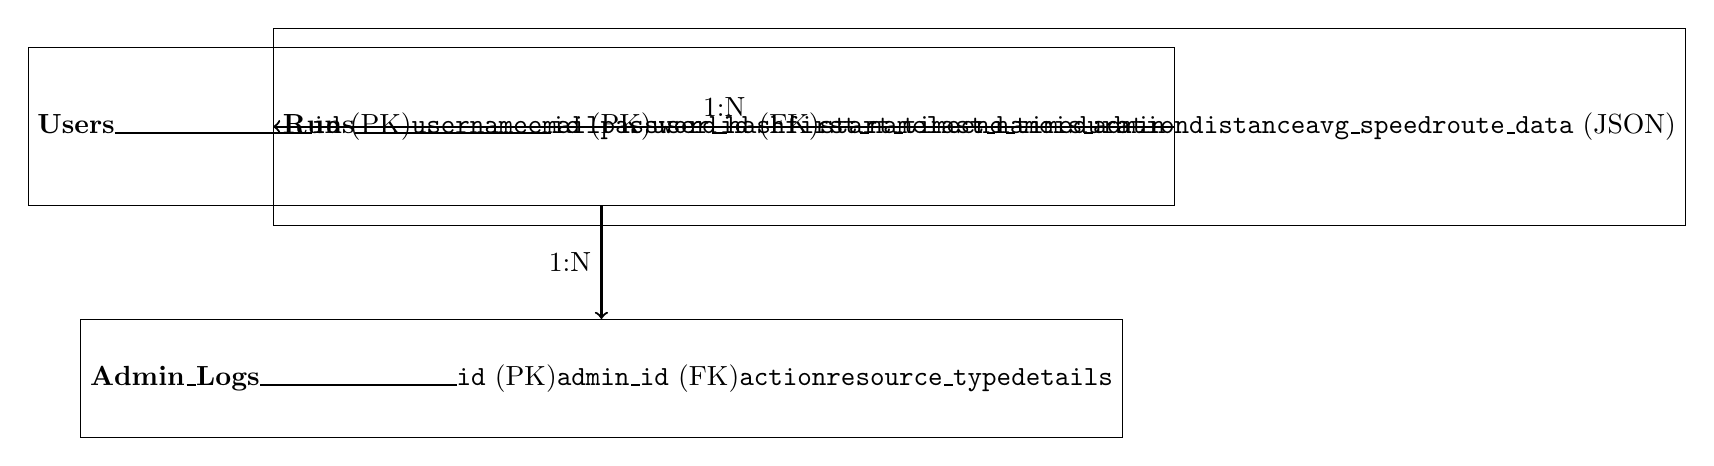
\begin{tikzpicture}[scale=0.8]
    % Users table
    \node[draw, rectangle, minimum width=3cm, minimum height=2cm] (users) at (0,0) {
        \textbf{Users}\\
        \rule{2.5cm}{0.4pt}\\
        \texttt{id} (PK)\\
        \texttt{username}\\
        \texttt{email}\\
        \texttt{password\_hash}\\
        \texttt{first\_name}\\
        \texttt{last\_name}\\
        \texttt{is\_admin}
    };
    
    % Runs table
    \node[draw, rectangle, minimum width=3cm, minimum height=2.5cm] (runs) at (6,0) {
        \textbf{Runs}\\
        \rule{2.5cm}{0.4pt}\\
        \texttt{id} (PK)\\
        \texttt{user\_id} (FK)\\
        \texttt{start\_time}\\
        \texttt{end\_time}\\
        \texttt{duration}\\
        \texttt{distance}\\
        \texttt{avg\_speed}\\
        \texttt{route\_data} (JSON)
    };
    
    % Admin logs table
    \node[draw, rectangle, minimum width=3cm, minimum height=1.5cm] (logs) at (0,-4) {
        \textbf{Admin\_Logs}\\
        \rule{2.5cm}{0.4pt}\\
        \texttt{id} (PK)\\
        \texttt{admin\_id} (FK)\\
        \texttt{action}\\
        \texttt{resource\_type}\\
        \texttt{details}
    };
    
    % Relations
    \draw[->, thick] (users.east) -- (runs.west) node[midway, above] {1:N};
    \draw[->, thick] (users.south) -- (logs.north) node[midway, left] {1:N};
    
\end{tikzpicture}
\caption{Diagramme Entité-Relations Simplifié}
\end{figure}

\subsection{Entités Principales}

\subsubsection{Entité User}

\begin{table}[H]
\centering
\begin{tabular}{|l|l|l|l|p{4cm}|}
\hline
\textbf{Champ} & \textbf{Type} & \textbf{Contraintes} & \textbf{Index} & \textbf{Description} \\
\hline
id & INTEGER & PK, AUTO\_INCREMENT & PRIMARY & Identifiant unique \\
username & VARCHAR(64) & UNIQUE, NOT NULL & INDEX & Nom d'utilisateur \\
email & VARCHAR(120) & UNIQUE, NOT NULL & INDEX & Adresse email \\
password\_hash & VARCHAR(128) & NOT NULL & - & Hash sécurisé du mot de passe \\
first\_name & VARCHAR(64) & NULL & - & Prénom \\
last\_name & VARCHAR(64) & NULL & - & Nom de famille \\
date\_of\_birth & DATE & NULL & - & Date de naissance \\
height & FLOAT & NULL & - & Taille en cm \\
weight & FLOAT & NULL & - & Poids en kg \\
is\_admin & BOOLEAN & DEFAULT FALSE & INDEX & Statut administrateur \\
created\_at & DATETIME & DEFAULT NOW() & INDEX & Date de création \\
updated\_at & DATETIME & DEFAULT NOW() & - & Dernière modification \\
\hline
\end{tabular}
\caption{Structure de la table Users}
\end{table}

\paragraph{Contraintes Métier}
\begin{itemize}
    \item Email doit respecter le format RFC 5322
    \item Username : 3-64 caractères alphanumériques
    \item Password hash : algorithme bcrypt avec salt
    \item Height : entre 100 et 250 cm si renseignée
    \item Weight : entre 30 et 200 kg si renseigné
\end{itemize}

\subsubsection{Entité Run}

\begin{table}[H]
\centering
\begin{tabular}{|l|l|l|l|p{4cm}|}
\hline
\textbf{Champ} & \textbf{Type} & \textbf{Contraintes} & \textbf{Index} & \textbf{Description} \\
\hline
id & INTEGER & PK, AUTO\_INCREMENT & PRIMARY & Identifiant unique \\
user\_id & INTEGER & FK, NOT NULL & INDEX & Référence utilisateur \\
start\_time & DATETIME & NOT NULL & INDEX & Début de la course \\
end\_time & DATETIME & NULL & - & Fin de la course \\
duration & INTEGER & NULL & - & Durée en secondes \\
distance & FLOAT & NULL & INDEX & Distance en mètres \\
avg\_speed & FLOAT & NULL & - & Vitesse moyenne (m/s) \\
max\_speed & FLOAT & NULL & - & Vitesse maximale (m/s) \\
calories & INTEGER & NULL & - & Calories brûlées \\
route\_data & JSON & NULL & - & Coordonnées GPS \\
created\_at & DATETIME & DEFAULT NOW() & INDEX & Date création \\
updated\_at & DATETIME & DEFAULT NOW() & - & Dernière modification \\
\hline
\end{tabular}
\caption{Structure de la table Runs}
\end{table}

\paragraph{Contraintes Métier}
\begin{itemize}
    \item Duration : calculé automatiquement si start\_time et end\_time présents
    \item Distance : minimum 10 mètres, maximum 500 km
    \item Avg\_speed : calculé à partir distance/durée
    \item Route\_data : tableau JSON de coordonnées \{lat, lng, timestamp\}
    \item Calories : estimation basée sur distance et profil utilisateur
\end{itemize}

\paragraph{Structure JSON Route Data}
\begin{lstlisting}[language=json]
[
    {
        "latitude": 48.856614,
        "longitude": 2.3522219,
        "altitude": 35.2,
        "timestamp": "2024-01-15T08:00:00Z",
        "accuracy": 5.0
    },
    {
        "latitude": 48.857614,
        "longitude": 2.3532219,
        "altitude": 36.1,
        "timestamp": "2024-01-15T08:00:05Z",
        "accuracy": 4.8
    }
]
\end{lstlisting}

\subsubsection{Entité Admin\_Logs}

\begin{table}[H]
\centering
\begin{tabular}{|l|l|l|l|p{4cm}|}
\hline
\textbf{Champ} & \textbf{Type} & \textbf{Contraintes} & \textbf{Index} & \textbf{Description} \\
\hline
id & INTEGER & PK, AUTO\_INCREMENT & PRIMARY & Identifiant unique \\
admin\_id & INTEGER & FK, NOT NULL & INDEX & Administrateur \\
action & VARCHAR(50) & NOT NULL & INDEX & Type d'action \\
resource\_type & VARCHAR(50) & NOT NULL & INDEX & Type de ressource \\
resource\_id & INTEGER & NULL & INDEX & ID de la ressource \\
details & TEXT & NULL & - & Détails de l'action \\
created\_at & DATETIME & DEFAULT NOW() & INDEX & Date de l'action \\
\hline
\end{tabular}
\caption{Structure de la table Admin\_Logs}
\end{table}

\subsection{Relations et Cardinalités}

\subsubsection{Relations Principales}

\begin{description}
    \item[\textbf{User ↔ Run}] Un utilisateur peut avoir plusieurs courses (1:N)
    \item[\textbf{User ↔ Admin\_Log}] Un administrateur peut effectuer plusieurs actions (1:N)
\end{description}

\subsubsection{Clés Étrangères et Intégrité}

\begin{lstlisting}[language=sql]
-- Contrainte d'intégrité référentielle
ALTER TABLE runs 
ADD CONSTRAINT fk_runs_user_id 
FOREIGN KEY (user_id) REFERENCES users(id) 
ON DELETE CASCADE ON UPDATE CASCADE;

-- Index composé pour les requêtes fréquentes
CREATE INDEX idx_runs_user_date 
ON runs(user_id, start_time DESC);

-- Index pour les recherches par période
CREATE INDEX idx_runs_timerange 
ON runs(start_time, end_time);
\end{lstlisting}

\subsection{Modèle Physique Optimisé}

\subsubsection{Stratégies d'Indexation}

\begin{table}[H]
\centering
\begin{tabular}{|l|l|l|p{5cm}|}
\hline
\textbf{Table} & \textbf{Index} & \textbf{Type} & \textbf{Justification} \\
\hline
users & idx\_users\_email & UNIQUE & Connexion par email \\
users & idx\_users\_username & UNIQUE & Connexion par username \\
runs & idx\_runs\_user\_date & COMPOSITE & Courses par utilisateur/date \\
runs & idx\_runs\_distance & SIMPLE & Recherche par distance \\
runs & idx\_runs\_timerange & COMPOSITE & Filtres temporels \\
admin\_logs & idx\_logs\_admin\_date & COMPOSITE & Historique admin \\
\hline
\end{tabular}
\caption{Stratégie d'indexation}
\end{table}

\subsubsection{Partitioning Strategy}

Pour une montée en charge future, le partitioning par date est envisagé :

\begin{lstlisting}[language=sql]
-- Partitioning par mois pour la table runs
CREATE TABLE runs (
    -- colonnes...
) PARTITION BY RANGE (YEAR(start_time) * 100 + MONTH(start_time)) (
    PARTITION p202401 VALUES LESS THAN (202402),
    PARTITION p202402 VALUES LESS THAN (202403),
    -- ...
);
\end{lstlisting}

\subsection{Calculs et Agrégations}

\subsubsection{Statistiques Utilisateur}

\begin{lstlisting}[language=sql]
-- Vue matérialisée pour les statistiques utilisateur
CREATE VIEW user_stats AS
SELECT 
    u.id,
    COUNT(r.id) as total_runs,
    COALESCE(SUM(r.distance), 0) as total_distance,
    COALESCE(SUM(r.duration), 0) as total_duration,
    COALESCE(AVG(r.avg_speed), 0) as overall_avg_speed,
    COALESCE(MAX(r.max_speed), 0) as personal_best_speed,
    COALESCE(SUM(r.calories), 0) as total_calories
FROM users u
LEFT JOIN runs r ON u.id = r.user_id
GROUP BY u.id;
\end{lstlisting}

\subsubsection{Performances et Tendances}

\begin{lstlisting}[language=sql]
-- Calcul de l'évolution des performances
SELECT 
    user_id,
    DATE(start_time) as run_date,
    distance,
    duration,
    (duration / distance * 1000) as pace_per_km,
    LAG(duration / distance * 1000) 
        OVER (PARTITION BY user_id ORDER BY start_time) as previous_pace
FROM runs
WHERE distance > 0 AND duration > 0
ORDER BY user_id, start_time;
\end{lstlisting}

\subsection{Migration et Évolution}

\subsubsection{Versioning du Schéma}

\begin{lstlisting}[language=python]
# Flask-Migrate pour les migrations automatiques
flask db init
flask db migrate -m "Initial migration"
flask db upgrade

# Migration type : ajout d'une colonne
flask db migrate -m "Add elevation data to runs"
\end{lstlisting}

\subsubsection{Compatibilité Descendante}

\begin{itemize}
    \item Ajout de colonnes avec valeurs par défaut
    \item Suppression différée avec marquage deprecated
    \item Scripts de migration de données
    \item Tests automatisés des migrations
\end{itemize}

\subsection{Backup et Archivage}

\subsubsection{Stratégie de Sauvegarde}

\begin{itemize}
    \item \textbf{Backup quotidien} : mysqldump complet
    \item \textbf{Backup incrémental} : binlog MySQL toutes les heures  
    \item \textbf{Archivage} : données de plus de 2 ans vers stockage froid
    \item \textbf{Tests de restoration} : validation mensuelle
\end{itemize}

\subsubsection{Politique de Rétention}

\begin{description}
    \item[\textbf{Données courantes}] Accès temps réel (< 6 mois)
    \item[\textbf{Données historiques}] Accès différé (6 mois - 2 ans)
    \item[\textbf{Données archivées}] Stockage long terme (> 2 ans)
    \item[\textbf{Suppression}] Sur demande utilisateur (RGPD)
\end{description}